\subsection{Loss functions}
\label{loss-functions}


\subsubsection{Common Loss Functions}
% Common loss functions
The most commonly used loss function for regression problem is the 
\textbf{Mean Squared Error (MSE)} function in \autoref{eq:mean-squared-error}.
It is the mathematically preferred function if the target distribution is Guassian.
It punishes large errors much more harshly than smaller errors, due to its squaring of the error.
\begin{equation}
  \label{eq:mean-squared-error}
  MSE = \frac{1}{n} \sum_{t=1}^n e_t^2
\end{equation}

If the target distribution consists of outliers, then the 
\textbf{Mean Absolute Error (MAE)} in \autoref{eq:mean-absolute-error} is more appropriate
as it does not punish the outliers too much.

\begin{equation}
  \label{eq:mean-absolute-error}
  MSE = \frac{1}{n} \sum_{t=1}^n |e_t|
\end{equation}

\subsubsection{ DILATE }

% Time and shape distortion
Both MAE and MSE are proven to be robust loss functions for regular regression problems,
but a paper published by \citeauthor{Guen2019} highligts some problems when the shape of the target function matters
such as in time series.
\autoref{fig:dilate} shows three different fits to the same target function, that all have
the same MSE error.

\begin{figure}[h!]
  \centering
  \begin{subfigure}[b]{0.3\textwidth}
    \centering
    \caption{Non informative prediction}
    \label{fig:dilate-non-informative}
    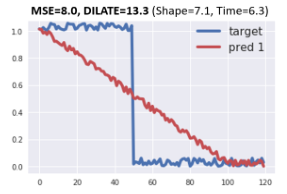
\includegraphics[width=\textwidth]{./figs/illustrations/dilate_ex1.png}
    \hfill
  \end{subfigure}

  \begin{subfigure}[b]{0.3\textwidth}
    \centering
    \caption{Correct shape, but with time delay}
    \label{fig:dilate-correct-shape}
    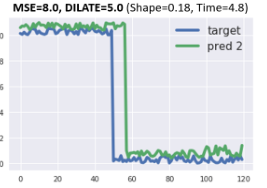
\includegraphics[width=\textwidth]{./figs/illustrations/dilate_ex2.png}
    \hfill
  \end{subfigure}
  \begin{subfigure}[b]{0.3\textwidth}
    \centering
    \caption{Correct time, but inaccurate shape}
    \label{fig:dilate-correct-time}
    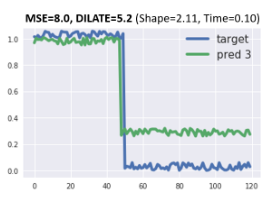
\includegraphics[width=\textwidth]{./figs/illustrations/dilate_ex3.png}
    \hfill
  \end{subfigure}
  \caption{Three examples of different shapes but same MSE error \citep{Guen2019}}
  \label{fig:dilate}
\end{figure}

In order to battle this problem they introduce a new loss function they call 
\textbf{DILATE (Distrortion Loss including Shape and Time)} \cite{Guen2019}.
DILATE uses a Neural Network instead of a mathematical function. 
It aims at accurately predicting sudden chanes, and explicitly incorporates two terms
supporting precise shape and temporal change detection.

The paper concludes that DILATE is comparable to the standard MSE loss when evaluated on MSE,
and far better when evaluated on time and shape metrics.


% Extreme value loss functions
\subsubsection{EVL}
\citeauthor{Ding2019} wrote a paper in 2019 regarding modern deep learning methods and their
weak perfomance when applied to real world time series, because their inability to predict extreme values.

Their deduction of why modern methods are unsatisfactory is bevause of the quadratic loss in 
the MSE loss function.
They take inspiration from \textit{Extreme Value Theory}, and develops a new kind of loss function
which they call \textbf{Extreme Value Loss (EVL)}.
They employ a memory network in order to memorize extreme events in historical records.

\autoref{fig:evl} show two fitted time series from the papers results. They conclude
that the method is superior to state of the art methods in extreme event detection, and 
in time series prediction.
\todo{Skrive litt mer detaljert om dette?}

\begin{figure}[h!]
  \centering
  \begin{subfigure}[b]{0.5\textwidth}
    \centering
    \caption{Output from GRU}
    \label{fig:evl-example1}
    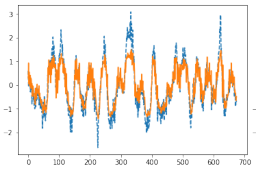
\includegraphics[width=\textwidth]{./figs/illustrations/evl_example1.png}
    \hfill
  \end{subfigure}

  \begin{subfigure}[b]{0.5\textwidth}
    \centering
    \caption{Output from EVL model}
    \label{fig:evl-example2}
    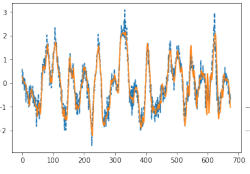
\includegraphics[width=\textwidth]{./figs/illustrations/evl_example2.png}
    \hfill
  \end{subfigure}
  \caption{Figures from \cite{Ding2019}}
  \label{fig:evl}
\end{figure}
